% -*- coding: utf-8; -*-

\chapter{Geração Baseada em Derivadas Médias}
\label{ch:my}
	Este capítulo descreve o método automático para gerar funções de transferência, proposto nesta dissertação, utilizando derivadas médias baseadas no trabalho de \textit{Kindlmann e Durkin}~\cite{gordon}.

\section{Detecção de Fronteiras}
\label{sec:my.deriv}
	Para eliminar o problema de deslocamento em $ h(v) $ é preciso repensar o modelo de \textit{Kindlmann e Durkin}~\cite{gordon}. A segunda derivada possui um ponto de inflexão na mesma posição em que ela assume zero. Esse ponto de inflexão pode ser utilizado para identificar a fronteira sem ser através de $ f''(x) = 0 $. No entanto, como são encontrados três pontos de inflexão ao longo de $ f''(x) $, é preciso identificar aquele que ocorre quando $ f'(x) $ é máximo.
	
	Como os pontos de inflexão de uma função podem ser encontrados através dos extremos locais em sua derivada, a função $ f'''(x) $ foi avaliada. A Figura~\ref{fig:m_inflection} exibe as funções $ f'(x) $, $ f''(x) $ e $ f'''(x) $, bem como as ocorrências dos pontos de inflexão em $ f''(x) $ pelas linhas tracejadas. Na figura, observa-se que a posição antes identificada por $ f''(x) = 0 $, agora pode ser encontrada através do mínimo local em $ f'''(x) $. 
	
\begin{figure}[h]
	\centering
	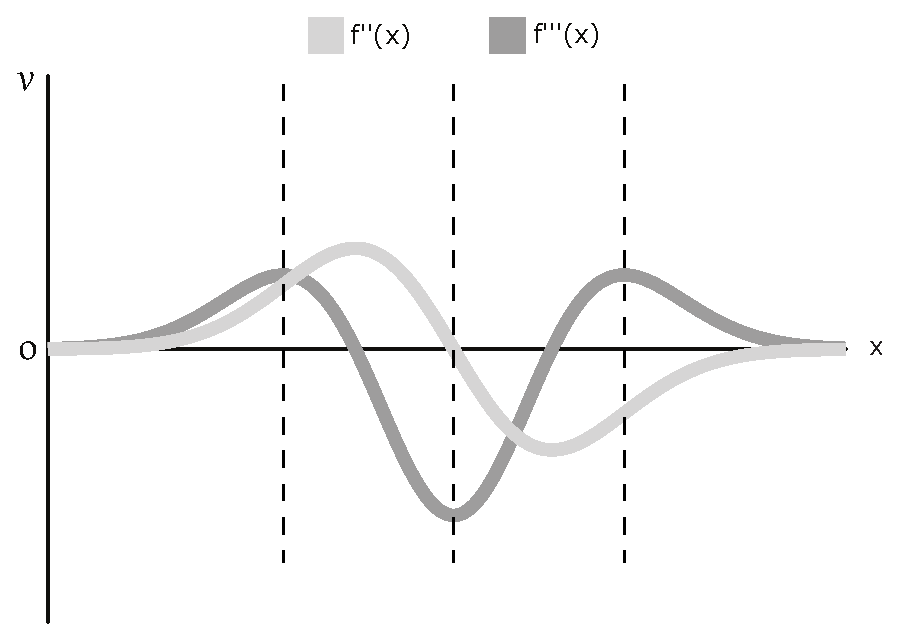
\includegraphics[width=0.7\textwidth]{images/m_inflection}
	\caption{Primeira, segunda e terceira derivadas na direção do gradiente, centradas na ocorrência de uma fronteira.}
	\label{fig:m_inflection}
\end{figure}

	No capítulo anterior foi visto que as derivadas médias $ g(v) $ e $ h(v) $ mantém os mesmos pontos característicos de $ f'(x) $ e $ f''(x) $ que identificam uma fronteira. Então, é preciso verificar que o mesmo ocorre com a terceira derivada média $ t(v) $. Para fazer tal demonstração, criou-se um volume sintético que consiste em duas esferas concêntricas, de raios e intensidades distintas, onde as fronteiras se comportam idealmente.
	
	A fatia do volume, exibida na Figura~\ref{fig:m_double_sphere}~\ref{fig:m_double_sphere_slice}, mostra que ele possui fronteiras nos intervalos $ [0,127] $ e $ [127,255] $. Portanto, espera-se que o centro das fronteiras estejam próximos a $ 64 $ e $ 190 $. Na Figura~\ref{fig:m_double_sphere}~\ref{fig:m_double_sphere_deriv} percebe-se que as derivadas médias se comportam exatamente como o esperado, pois $ 64 $ e $ 190 $ são justamente os pontos de primeira derivada máxima, segunda derivada zero e terceira derivada mínima.
	
\begin{figure}[h]
	\centering
	\subfigure[Fatia do volume]
	{
		
\includegraphics[width=0.3\textwidth]{images/m_double_sphere_slice}
		\label{fig:m_double_sphere_slice}
	}
	\subfigure[Derivadas médias do volume]
	{
		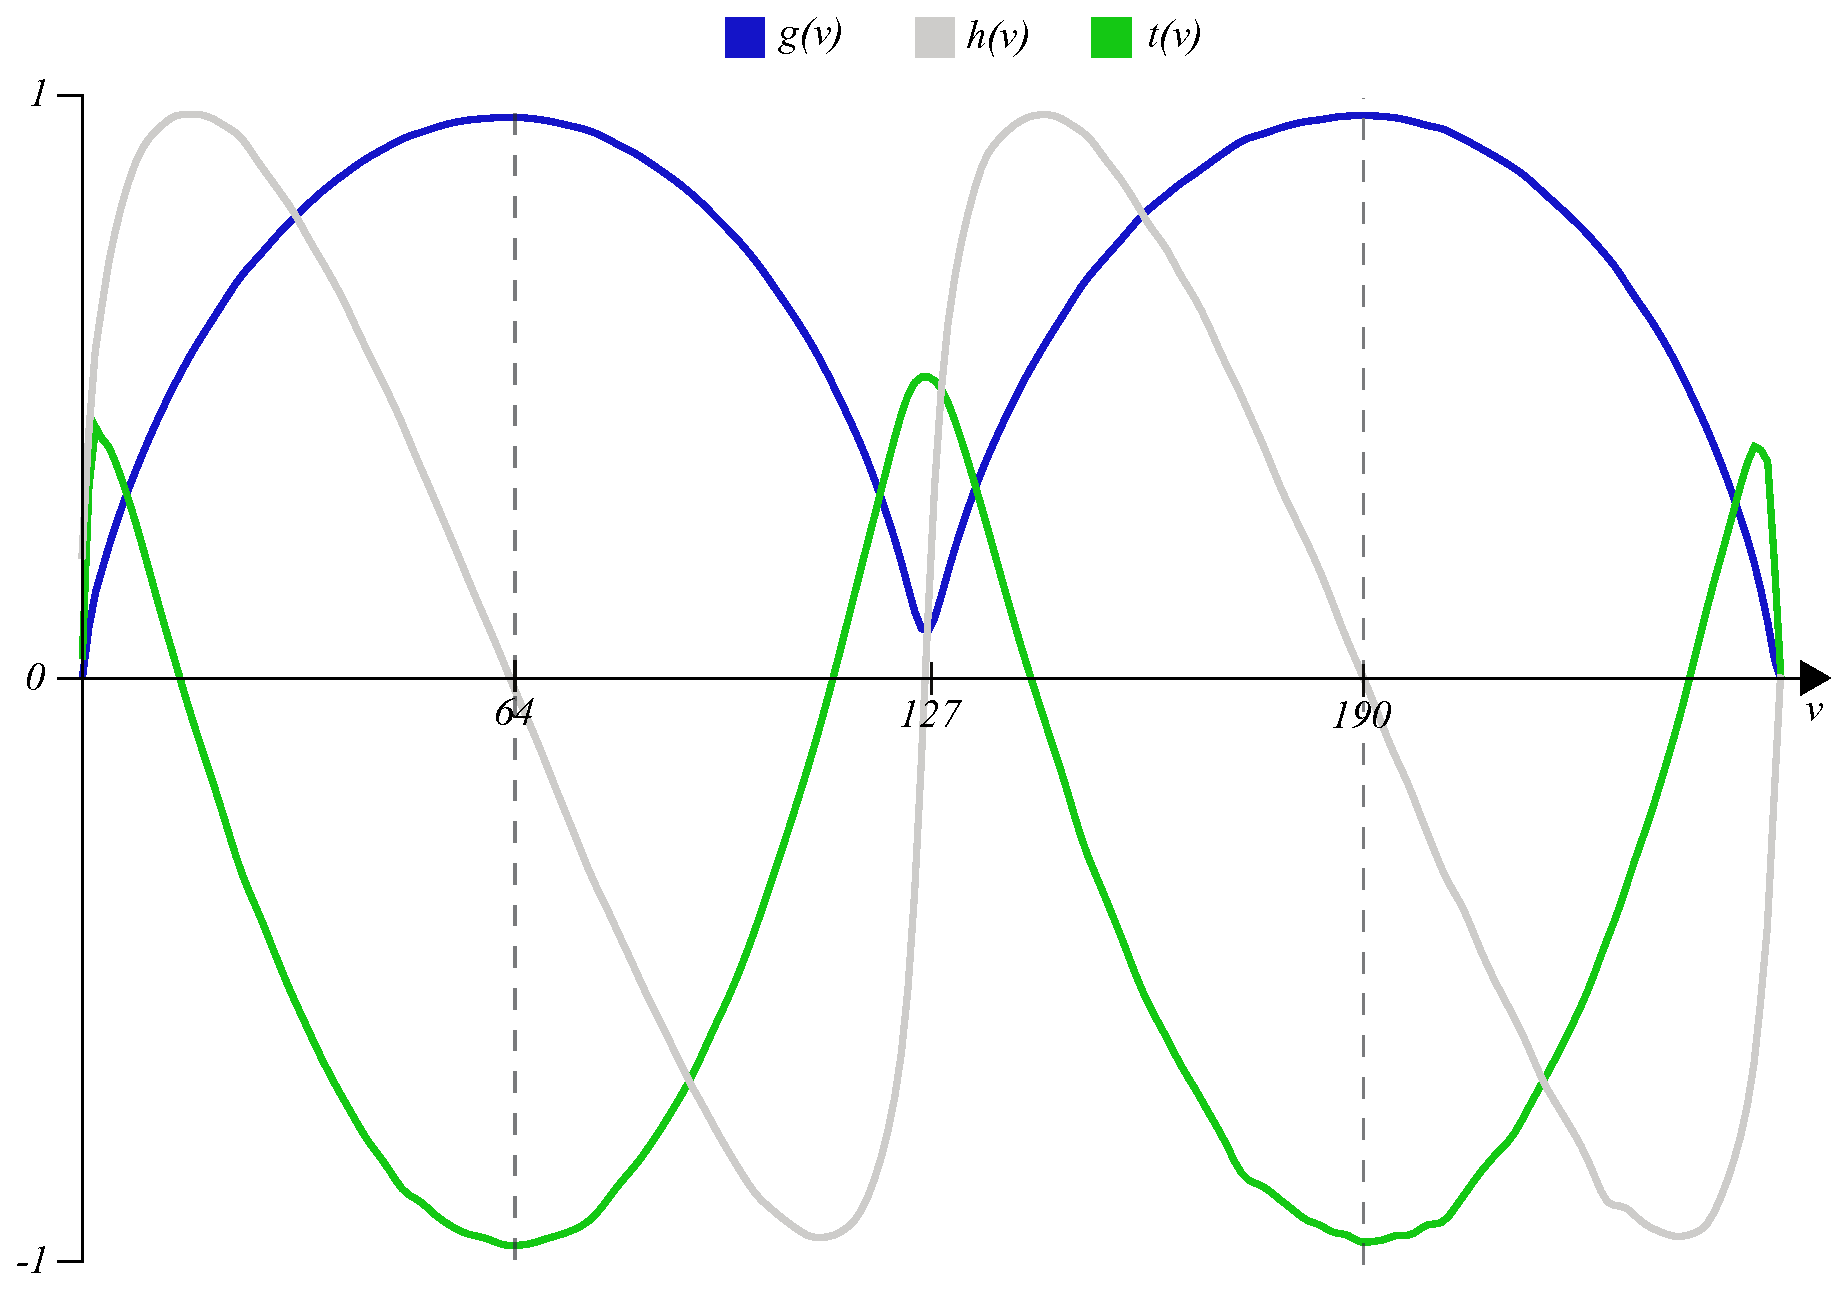
\includegraphics[width=0.6\textwidth]{images/m_double_sphere_derivatives}
		\label{fig:m_double_sphere_deriv}
	}
	\caption{Duas esferas concêntricas sem sobreposição no intervalo de valores das fronteiras.}
	\label{fig:m_double_sphere}
\end{figure}

	No entanto, $ h(v) $ é igual a zero em $ 127 $, indicando uma fronteira que não existe. Para este exemplo sintético e ideal, como o valor de $ g(v) $ é baixo, a função $ p(v) $ nesse ponto resulta em uma distância maior que a ocorrida em $ 64 $ e $ 190 $. Dessa forma, a fronteira falsa é sempre menos opaca que as fronteias reais no método de \textit{Kindlmann e Durkin}~\cite{gordon}, mas dependendo da função $ b(x) $ definida pelo usuário e do valor de $ g_{thresh} $, a falsa fronteira pode acabar sendo realçada e visualizada, como ilustra a Figura~\ref{fig:m_double_sphere_tf}.
	
	A visualização volumétrica apresentada na Figura~\ref{fig:m_double_sphere_tf}~\ref{fig:m_double_sphere_right}, que realça corretamente as fronteiras do volume, foi obtida com a função de transferência indicada na Figura~\ref{fig:m_double_sphere_tf}~\ref{fig:m_double_sphere_tf_right}, onde utilizou-se $ b(x) $ com largura igual a $ 1 $. No entanto, ao aumentar a largura de $ b(x) $ para $ 3 $, obtém-se uma FT com um novo comportamento, ilustrada na Figura~\ref{fig:m_double_sphere_tf}~\ref{fig:m_double_sphere_tf_wrong}. Como resultado, a nova visualização apresenta uma falsa fronteira em amarelo que pode ser vista na Figura~\ref{fig:m_double_sphere_tf}~\ref{fig:m_double_sphere_wrong}.

\begin{figure}[h]
	\centering
	\subfigure[]
	{
		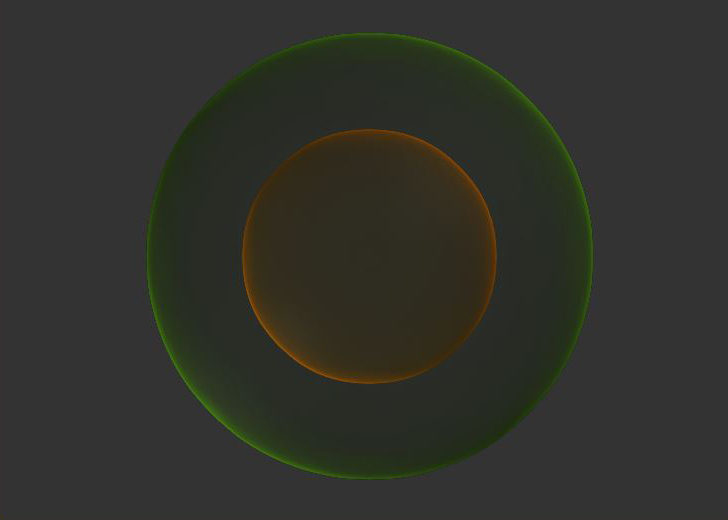
\includegraphics[width=0.4\textwidth]{images/m_double_sphere}
		\label{fig:m_double_sphere_right}
	}
	\subfigure[]
	{
		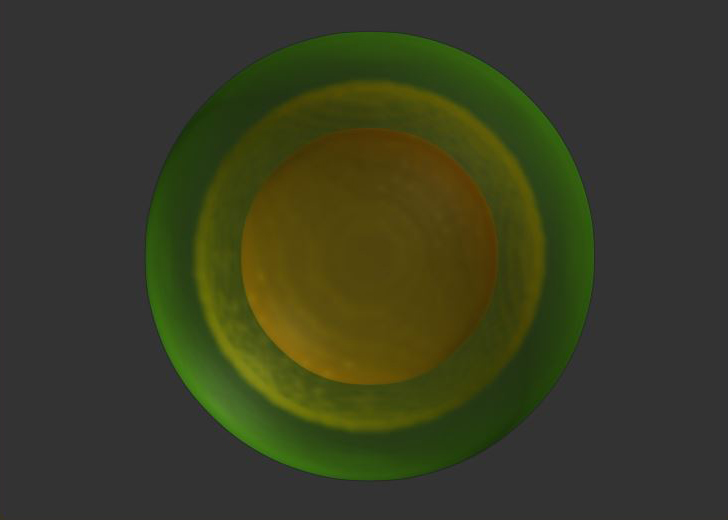
\includegraphics[width=0.4\textwidth]{images/m_double_sphere_wrong}
		\label{fig:m_double_sphere_wrong}
	}
	\subfigure[]
	{
		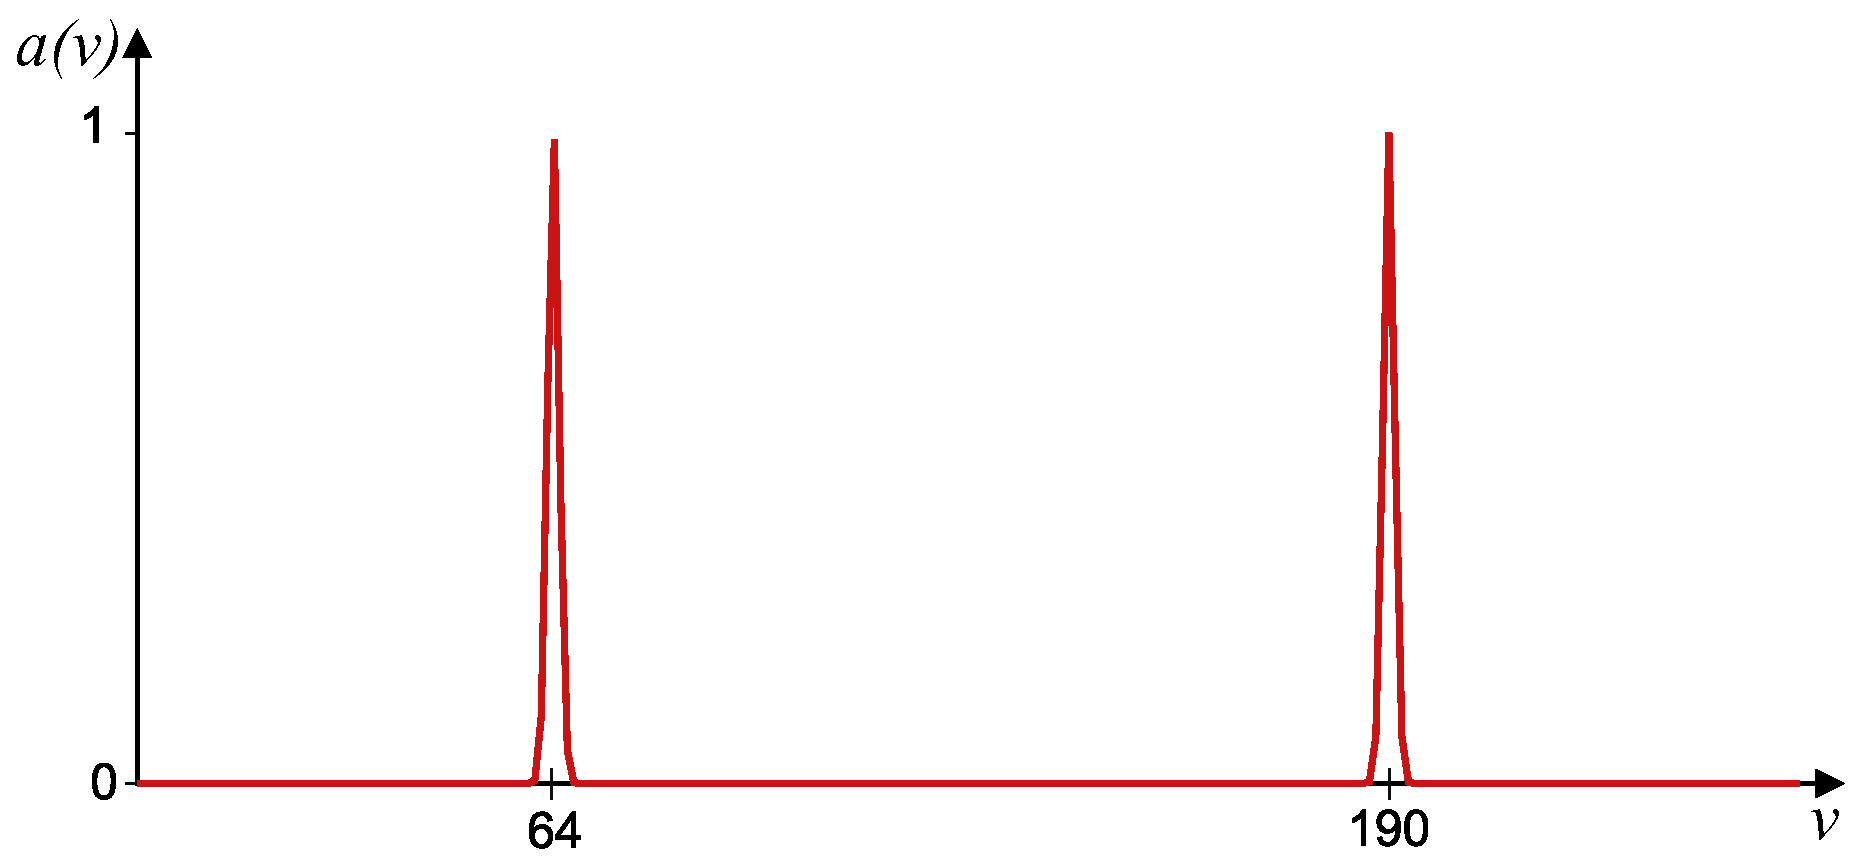
\includegraphics[width=0.7\textwidth]{images/m_double_sphere_tf_right}
		\label{fig:m_double_sphere_tf_right}
	}
	\subfigure[]
	{
		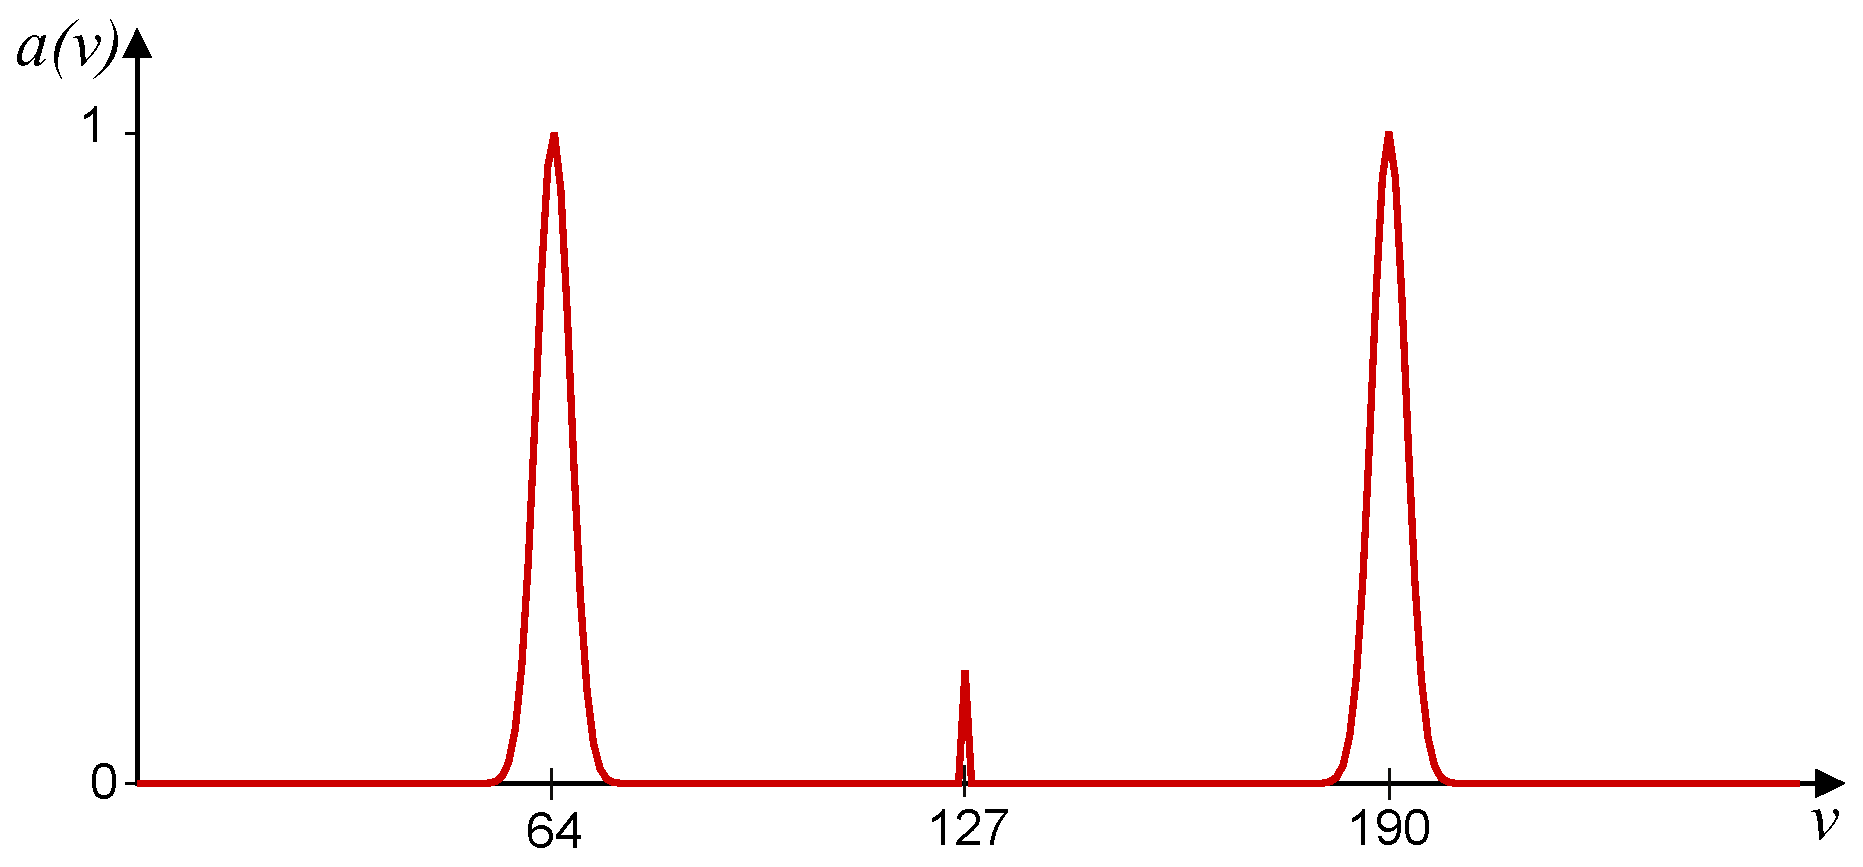
\includegraphics[width=0.7\textwidth]{images/m_double_sphere_tf_wrong}
		\label{fig:m_double_sphere_tf_wrong}
	}
	\caption{Duas esferas concêntricas sem sobreposição no intervalo de valores das fronteiras.}
	\label{fig:m_double_sphere_tf}
\end{figure}

	É preciso lembrar também que as funções $ g(v) $, $ h(v) $ e $ t(v) $ raramente apresentarão o comportamento exibido na Figura~\ref{fig:m_double_sphere}~\ref{fig:m_double_sphere_deriv}. Nos volumes em que o intervalo de valores das fronteiras se sobrepõem, a média afeta o comportamento dos arcos esperados. Para demonstrar esse fenômeno, outro volume sintético foi criado, também contendo duas esferas concêntricas, onde as fronteiras se comportam de forma ideal. Porém, neste segundo, o intervalo de valores das fronteiras se sobrepõem. A Figura~\ref{fig:m_double_sphere_disc} exibe uma fatia do volume e também suas derivadas médias.
	
	Como pode ser observado na Figura~\ref{fig:m_double_sphere_disc}~\ref{fig:m_double_sphere_disc_slice}, os intervalos das fronteiras são $ [0,255] $ e $ [170,255] $. Percebe-se que devido à sobreposição de valores, as funções não se comportam como o esperado. Apesar de existir uma fronteira entre $ 0 $ e $ 255 $, as derivadas não exibem um arco único entre esses valores. A Figura~\ref{fig:m_double_sphere_disc}~\ref{fig:m_double_sphere_disc_deriv} mostra que o arco é interrompido justamente no valor $ 170 $, que é o início da segunda fronteira e, por isso, um arco também destorcido se estende até $ 255 $.	
	
\begin{figure}[h]
	\centering
	\subfigure[Fatia do volume]
	{
		
\includegraphics[width=0.3\textwidth]{images/m_double_disc_sphere_slice}
		\label{fig:m_double_sphere_disc_slice}
	}
	\subfigure[Derivadas médias do volume]
	{
		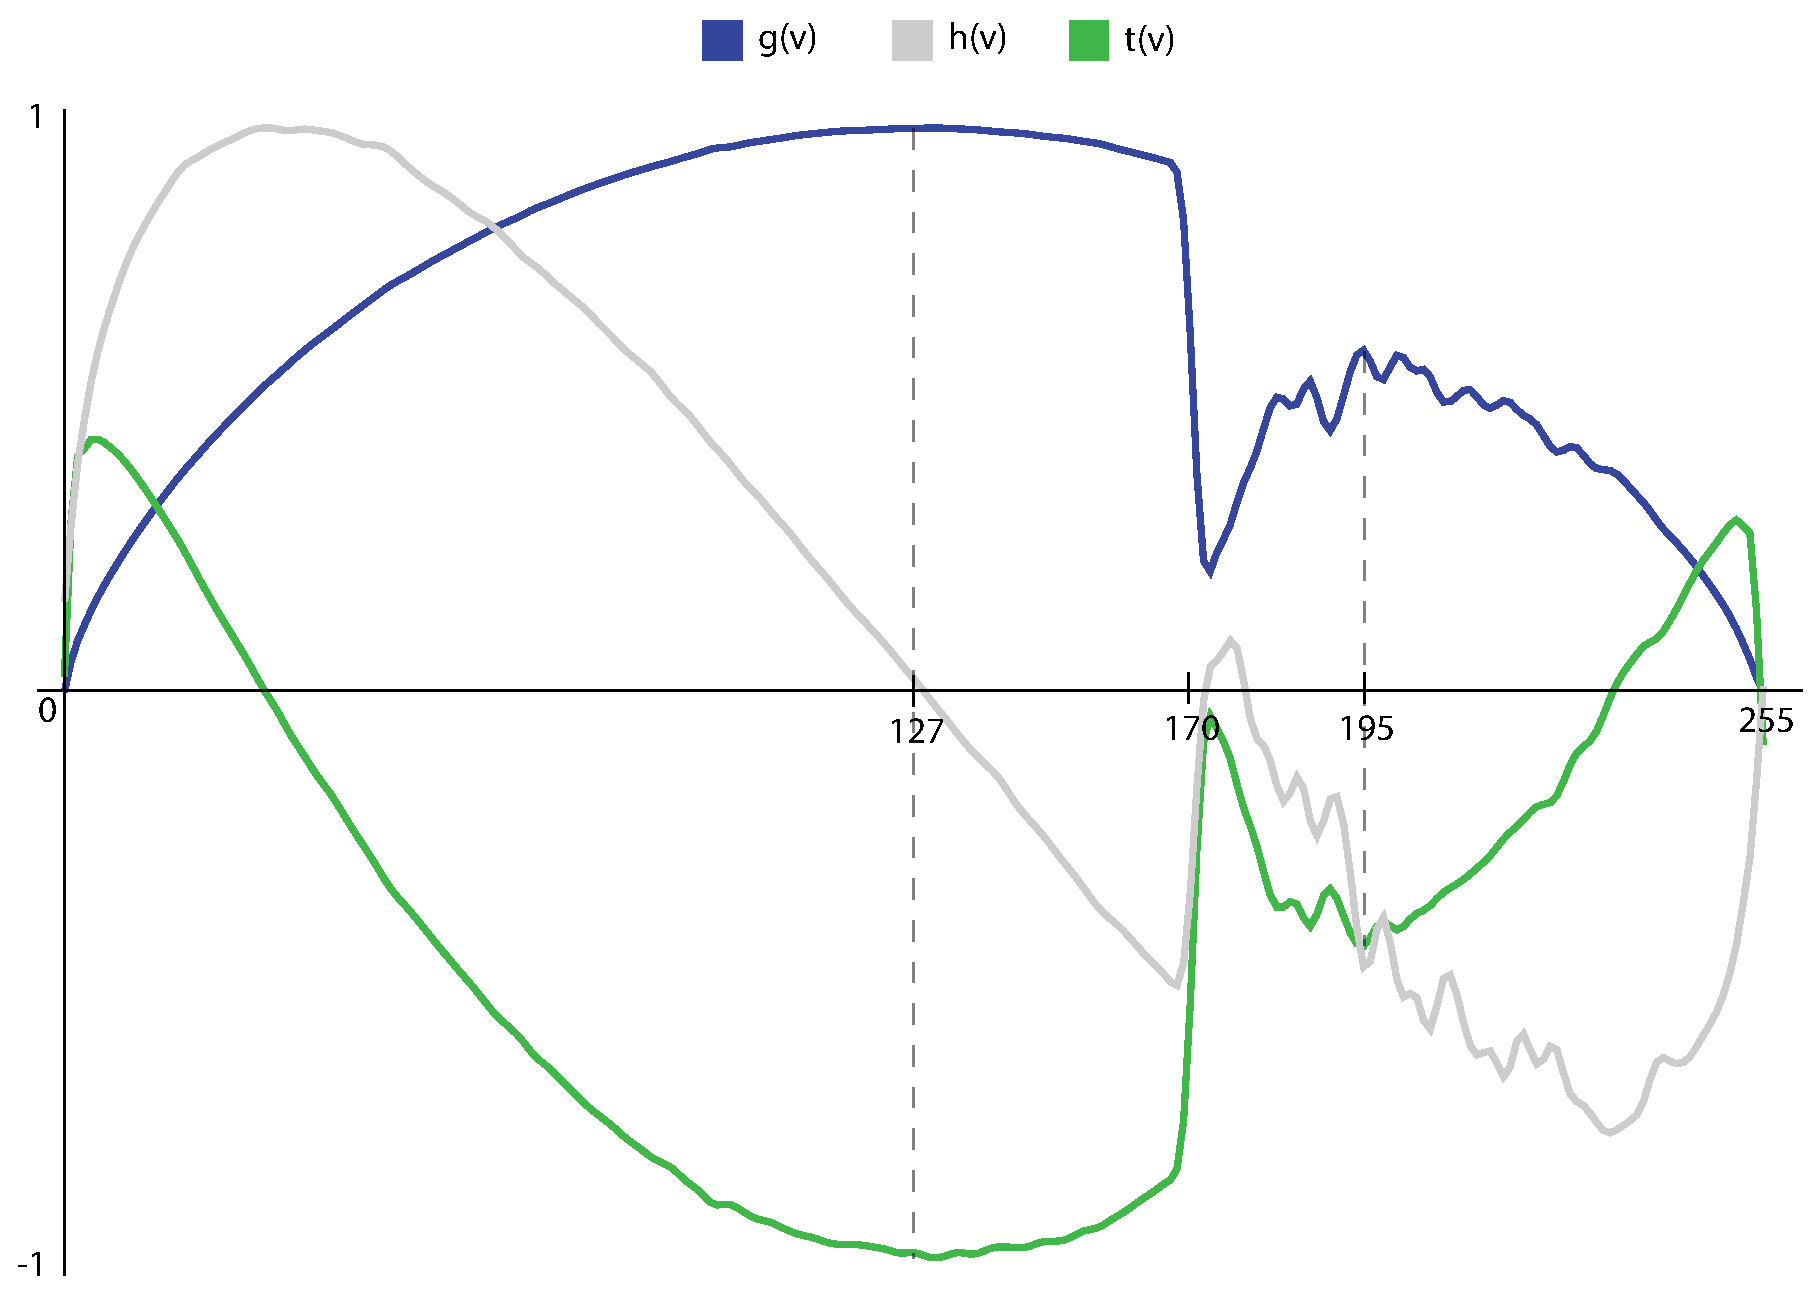
\includegraphics[width=0.6\textwidth]{images/m_double_disc_sphere_derivatives}
		\label{fig:m_double_sphere_disc_deriv}
	}
	\caption{Duas esferas concêntricas com sobreposição no intervalo de valores das fronteiras.}
	\label{fig:m_double_sphere_disc}
\end{figure}
	
	Dado os intervalos conhecidos das fronteiras, sabe-se que seus respectivos centros são próximos a $ 127 $ e $ 213 $. Em $ 127 $ vê-se que as três funções médias se comportam como esperado na ocorrência de uma fronteira. Porém, o mesmo não acontece em $ 213 $. As funções $ g(v) $ e $ t(v) $ apresentam extremos locais muito próximos, perto de $ 196 $. No entanto, $ h(v) $ não cruza o eixo em $ 213 $, nem em $ 196 $.
	
	Então, percebe-se que $ t(v) $ se comporta melhor que $ h(v) $ na presença de uma fronteira e que seu deslocamento devido à sobreposição nos intervalos das fronteiras é semelhante ao ocorrido em $ g(v) $. Contudo, para identificar uma fronteira a partir da terceira derivada é preciso obter uma nova relação para extrair $ \sigma $ e $ x $, mas agora utilizando $ f'(x) $ e $ f'''(x) $. Para facilitar a leitura, $ f'(x) $ é repetida na Equação~\eqref{eq:first2}, enquanto a função $ f'''(x) $ é definida na Equação~\eqref{eq:third}.
	
\begin{equation} \label{eq:first2}
g = f'(x) = \frac{v_{max} - v_{min}}{\sigma\sqrt{2\pi}}\ e^{-\frac{x^{2}}{2\sigma^{2}}}
\end{equation} \

\begin{equation} \label{eq:third}
t = f'''(x) = -\frac{(x^{2} - \sigma^{2})(v_{max} - v_{min})}{\sigma^{5}\sqrt{2\pi}}\ e^{-\frac{x^{2}}{2\sigma^{2}}}
\end{equation} \
	
	Devido ao fato de $ f'(x) $ ter um grande termo em comum com $ f'''(x) $, a simples divisão entre essas funções revela uma relação envolvendo $ \sigma $ e $ x $, como mostra a Equação~\eqref{eq:sigmax}. Com $ x = 0 $ percebe-se que, mais uma vez, o valor de $ \sigma $ pode ser recuperado através dos valores extremos das derivadas, indicado na Equação~\eqref{eq:sigma3}. Por fim, $ x $ pode ser isolado na Equação~\eqref{eq:sigmax} resultando em uma nova expressão para a distância ao centro da fronteira, indicada na Equação~\eqref{eq:x3}.

\begin{equation} \label{eq:sigmax}
	\frac{f'''(x)}{f'(x)} = \frac{x^{2} - \sigma^{2}}{\sigma^{4}}
\end{equation} \

\begin{equation} \label{eq:sigma3}
	\sigma^{2} = -\frac{f'(0)}{f'''(0)} \ \approx \ -\frac{g(v)_{max}}{t(v)_{min}}
\end{equation} \

\begin{equation} \label{eq:x3}
	x = \sigma^{2}\sqrt{\frac{f'''(x)}{f'(x)} + \frac{1}{\sigma^{2}}} \ \approx \ 
	p(v) = \sigma^{2}\sqrt{\frac{t(v)}{g(v)} + \frac{1}{\sigma^{2}}}
\end{equation} \\

	À primeira vista, o uso da terceira derivada no lugar da segunda garante que o deslocamento das curvas médias não resultará na atribuição de um $ v $ incorreto à fronteira. No entanto, isso ainda pode ocorrer indiretamente, a partir da distância $ x $. Uma análise da contribuição de $ \sigma $ para o valor de $ x $ ajuda a entender melhor essa relação.
	
	$ p(v) $ é igual a zero apenas quando $ \frac{t(v)}{g(v)} = -\frac{1}{\sigma^{2}} $, já que $ \sigma $ não pode ser zero. Como $ \sigma $ é obtido a partir dos valores extremos de $ g(v) $ e $ t(v) $, qualquer deslocamento nessas funções altera seu valor. Consequentemente, $ p(v) = 0 $ pode ocorrer em um $ v $ que não corresponde exatamente ao centro da fronteira. 
	
	A Figura~\ref{fig:m_sigma} ilustra como uma pequena variação no valor de $ \sigma $ pode ter um grande impacto na função de transferência. As curvas exibidas são referentes ao mesmo volume utilizado na Figura~\ref{fig:m_double_sphere}. O $ \sigma $ de valor $ 2,21 $ é o teoricamente correto, obtido através da Equação~\eqref{eq:sigma3}. A função de transferência resultante do uso deste $ \sigma $ realça muito mais a fronteira em $ 64 $ que em $ 190 $. Além disso, a FT em $ 64 $ apresenta um formato em \quote{U}, possuindo dois picos com um vale no meio onde deveria haver um só pico.
	
	Variando $ \sigma $ em apenas $ 0.02 $ vê-se que a função de transferência alterna entre realçar apenas a fronteira em $ 64 $, com baixa opacidade, e identificar as duas fronteiras apresentando um formato em \quote{U}, evidenciando que o $ \sigma $ pode provocar um deslocamento em $ p(v) $.
	
	A rigor, cada fronteira deveria possuir seu próprio sigma. De fato, durante a aquisição dos dados, o volume gerado incorpora um borrão uniforme, que ao ser representado por uma gaussiana implica em um único valor para $ \sigma $. No entanto, como diferentes fronteiras podem possuir espessuras distintas, nos casos em que o volume possui mais de uma fronteira, expressar essa espessura por um sigma único leva a uma função de transferência menos adequada.
	
	Mais estudos precisam ser feitos a fim de se distinguir a espessura de fronteiras distintas, matematicamente. Entretanto, ao invés de obter parâmetros para corrigir $ p(v) $, como \textit{Kindlmann e Durkin}~\cite{gordon} fizeram com $ g_{thresh} $, uma nova abordagem pode ser pensada para identificar fronteiras a partir dos valores extremos de $ f'(x) $ e $ f'''(x) $. Por exemplo, uma métrica pode ser desenvolvida para atribuir opacidade ao volume, baseada nos máximos e mínimos locais de $ g(v) $ e $ t(v) $.
	
\begin{figure}
	\centering
	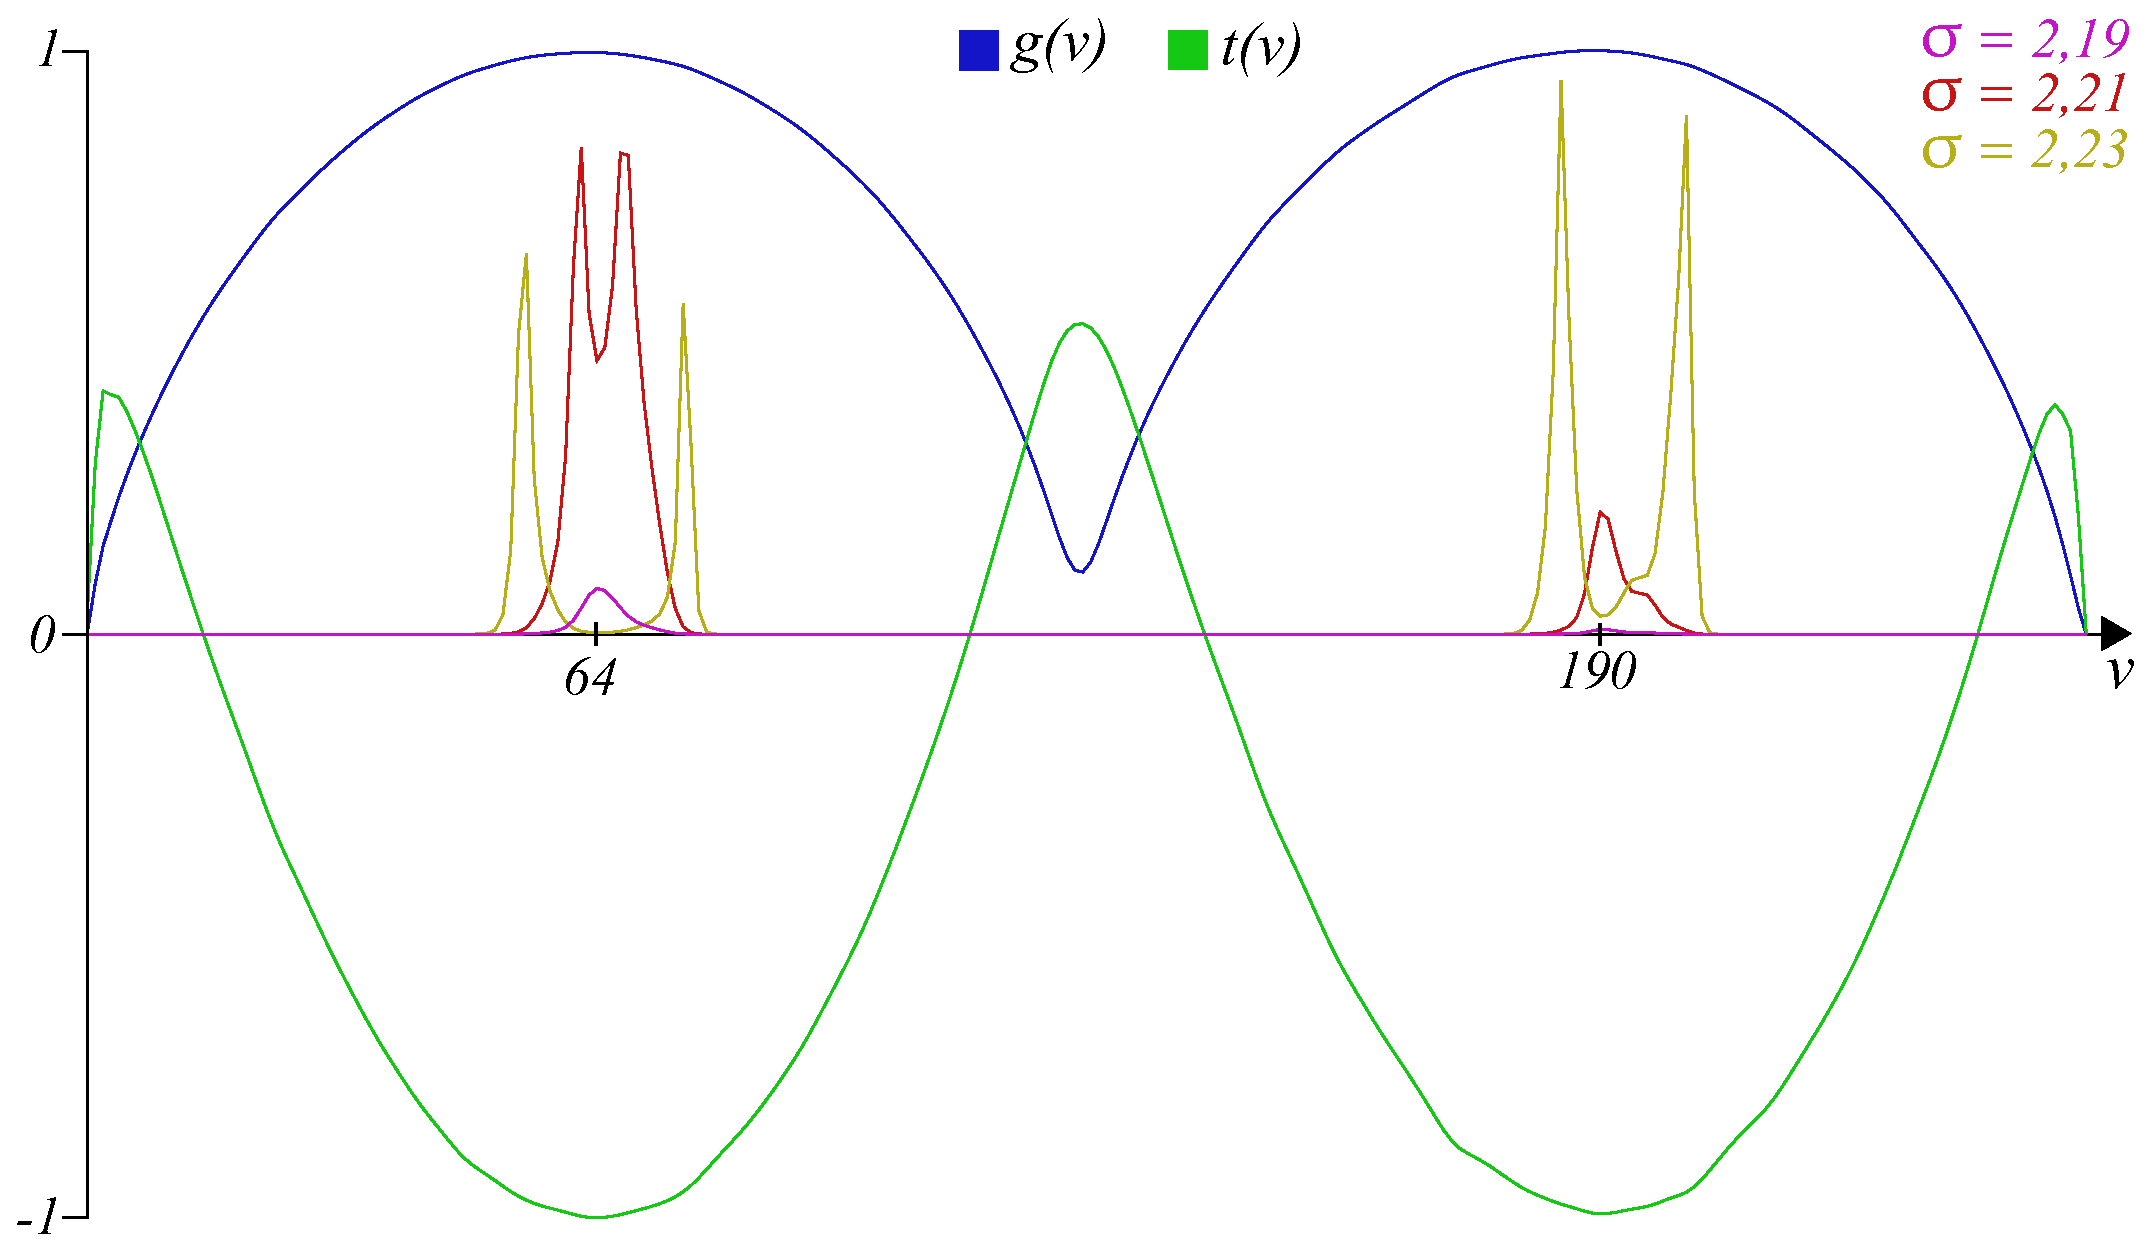
\includegraphics[width=0.8\textwidth]{images/m_sigma}
	\caption{O impacto da variação do $ \sigma $ na função de transferência.}
	\label{fig:m_sigma}
\end{figure}
	
	Como a terceira derivada é mais sensível que a primeira, ela possui uma curva mais expressiva em relação aos extremos locais. Essa característica faz com que a terceira derivada seja mais robusta em relação a falsos positivos, isto é, ela tende a apresentar menos extremos locais que não indicam uma fronteira, mas que existem em decorrência da média dos valores. Ao mesmo tempo, a terceira derivada conserva melhor seus extremos locais, não perdendo-os devido à suavização que é inerente quando se tira uma média.
	
\begin{figure}
	\centering
	\subfigure[Fatia do volume.]
	{
		
\includegraphics[width=0.2\textwidth]{images/m_triple_sphere_slice}
		\label{fig:m_triple_slice}
	}
	\subfigure[Funções $ g(v) $ e $ t(v) $.]
	{
		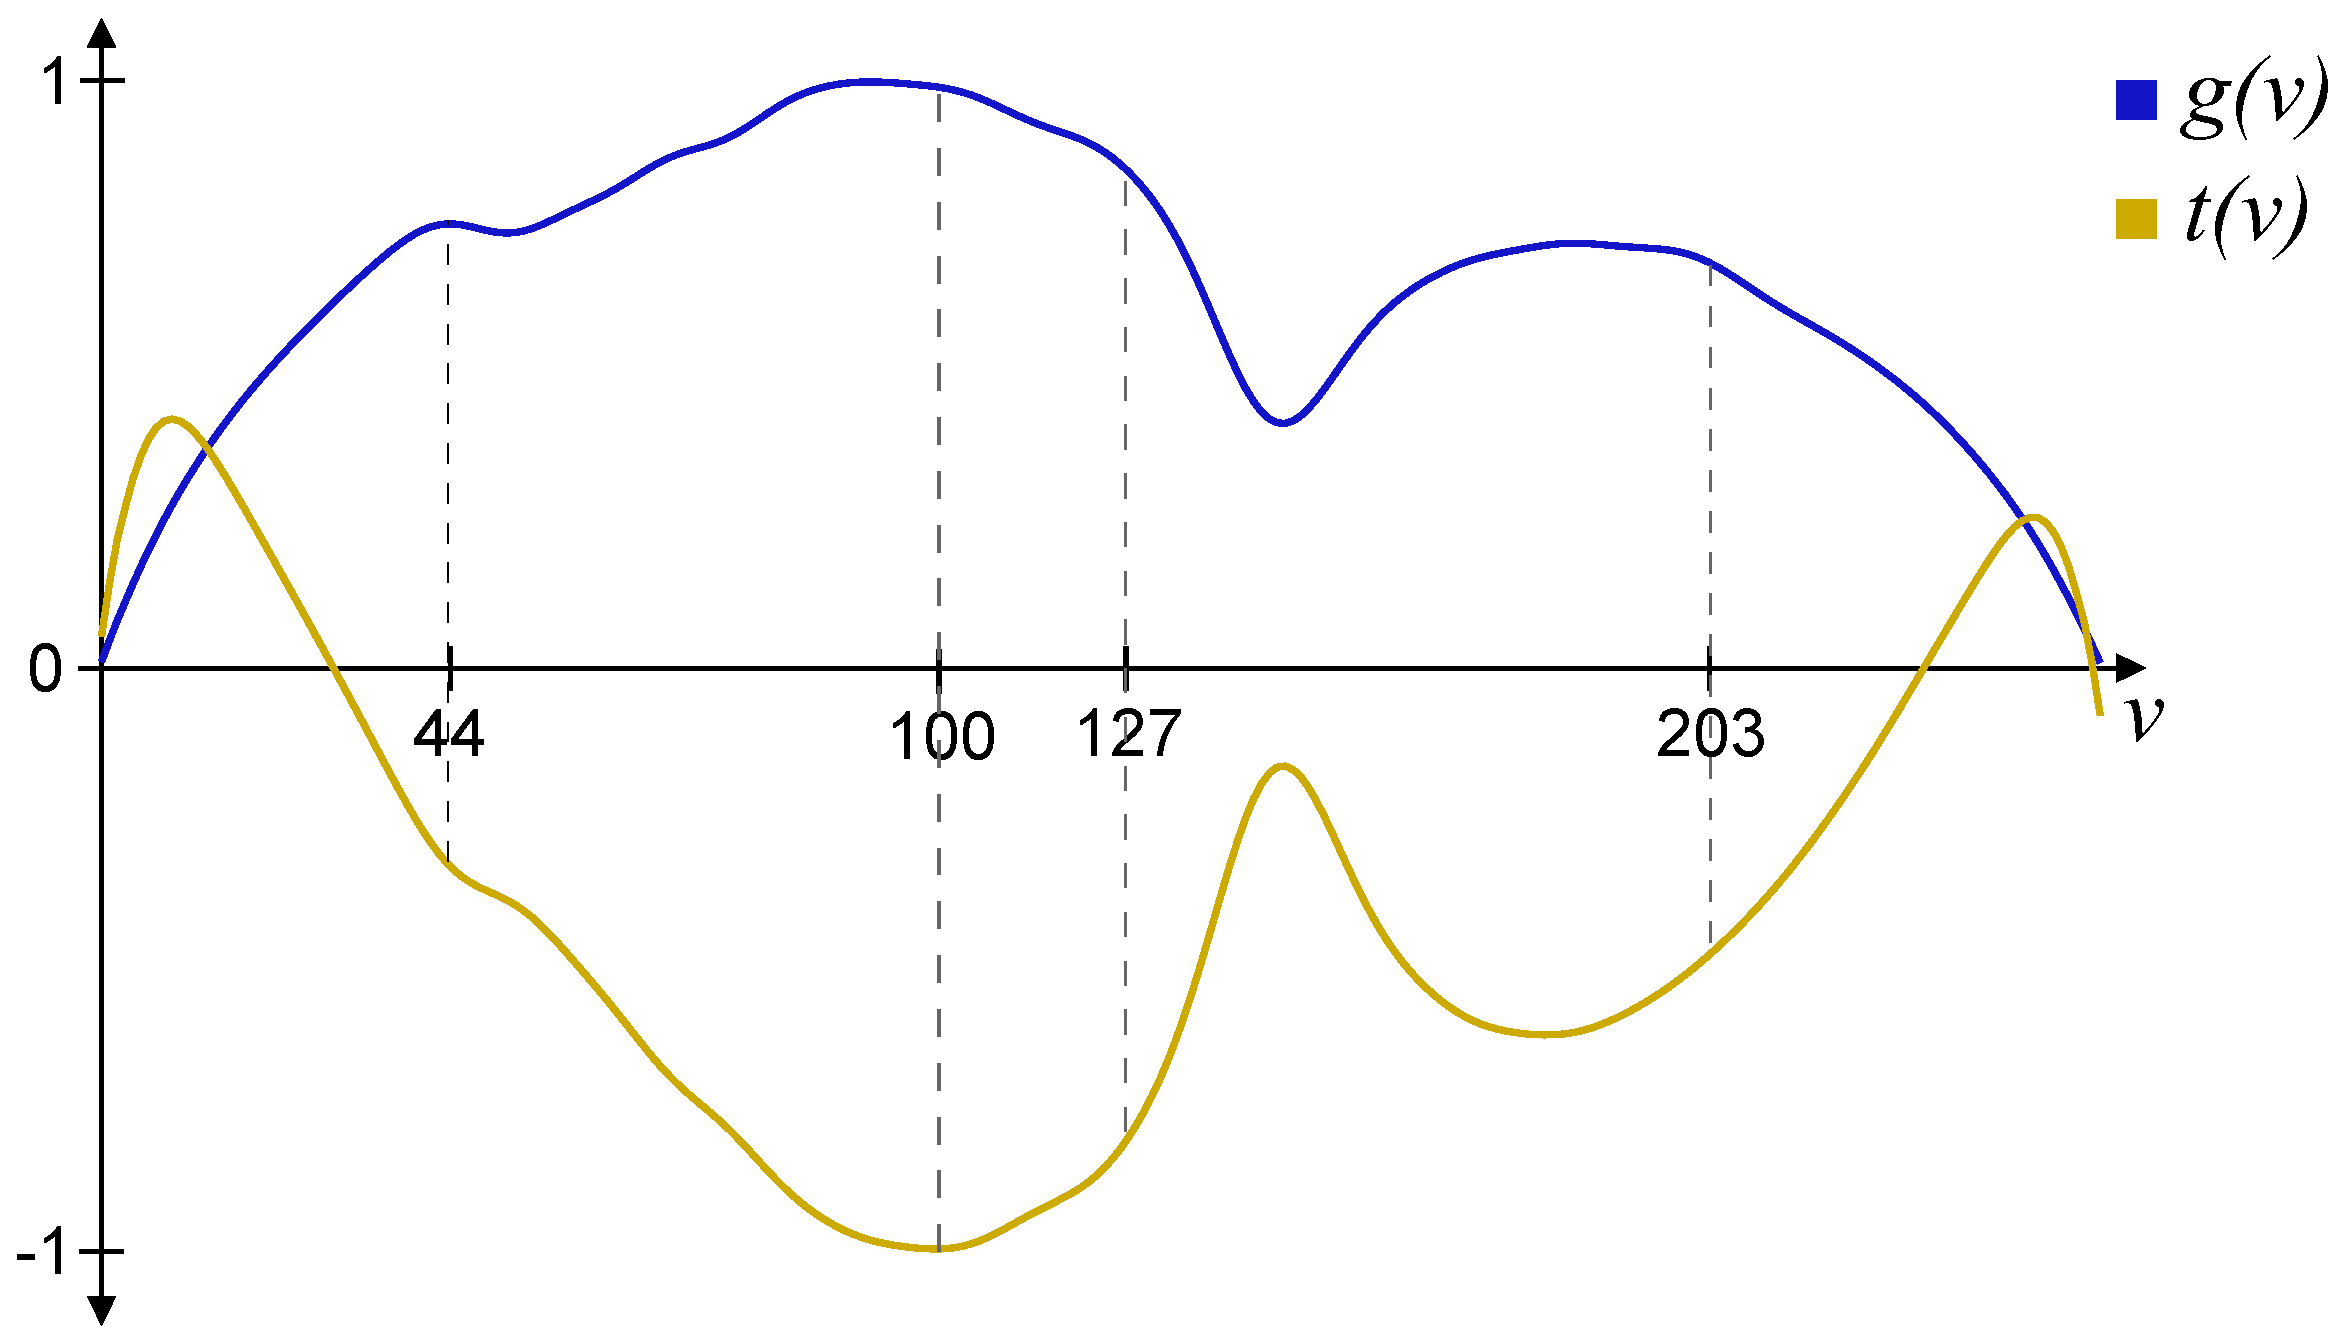
\includegraphics[width=0.7\textwidth]{images/m_triple_sphere_ft}
		\label{fig:m_triple_ft}
	}
	\caption{Volume sintético composto por três esferas concêntricas.}
	\label{fig:m_triple}
\end{figure}
	
	Um volume sintético composto por três esferas concêntricas foi utilizado para ilustrar como as derivadas médias podem exibir quantidades diferentes de extremos locais. Uma fatia do volume, exibida na Figura~\ref{fig:m_triple}~\ref{fig:m_triple_slice}, mostra que existem três fronteiras nos seguintes intervalos: $ [0,255] $, $ [50,150] $ e $ [150,255] $. Portanto, as fronteiras estão próximas a $ 128 $, $ 100 $ e $ 203 $, respectivamente. Como pode ser visto na Figura~\ref{fig:m_triple}~\ref{fig:m_triple_ft}, a primeira derivada apresenta um extremo local em $ 44 $ que não corresponde a uma fronteira. O mesmo não ocorre com a terceira derivada.
	
	Então, escolheu-se utilizar simplesmente os mínimos locais de $ t(v) $ para identificar o centro das fronteiras. Além de eliminar o $ g_{thresh} $, o resultado desta abordagem é uma função de transferência composta por um conjunto de funções de opacidade atribuídas às isosuperfícies mais importantes do volume. Essa característica permite que o usuário escolha quais fronteiras deseja visualizar. 
	
	Na Seção~\ref{sec:my.tf} a métrica exata de como gerar a função de transferência será descrita. As subseções abaixo apresentam como calcular a terceira derivada do volume de dados.
	
\subsection{Cálculo das Derivadas}
	Para calcular as derivadas é preciso lembrar que o volume não possui uma função analítica $ f(x, y, z) $ que o defina. Ele contém apenas um mapeamento de uma posição $ (x, y, z) $ para um valor escalar $ v $. Portanto, as derivadas de cada ponto do volume precisam ser calculadas com base na sua vizinhança e esse cálculo pode variar de acordo com o tipo do volume de dados.
	
	Se um volume pode ser representado por uma malha regular, então ele é espacialmente delimitado por uma caixa retangular, preenchida por células cúbicas alinhadas aos eixos da caixa, onde cada célula representa um dado do volume. Este é o caso dos volumes resultantes da maioria dos métodos de aquisição por escaneamento de uma estrutura fisiológica real, como os exames médicos. Há ainda volumes cujos dados são topologicamente estruturados, mas que não podem ser representados por uma grade regular, pois a direção da disposição dos dados varia ao longo do volume. Então, utiliza-se uma malha não regular, composta por células hexaédricos irregulares, como é o caso dos volumes resultantes das simulações de reservatórios de petróleo utilizados nesta dissertação.
	
	A diferença entre esses dois tipos de representatividade pode ser vista na Figura~\ref{fig:meshes}, onde uma versão 2D de cada malha é ilustrada. O modo de se calcular as derivadas para cada um desses casos é discutido nas subseções seguintes.
	
\begin{figure}[h]
	\centering
	\subfigure[Malha regular]
	{
		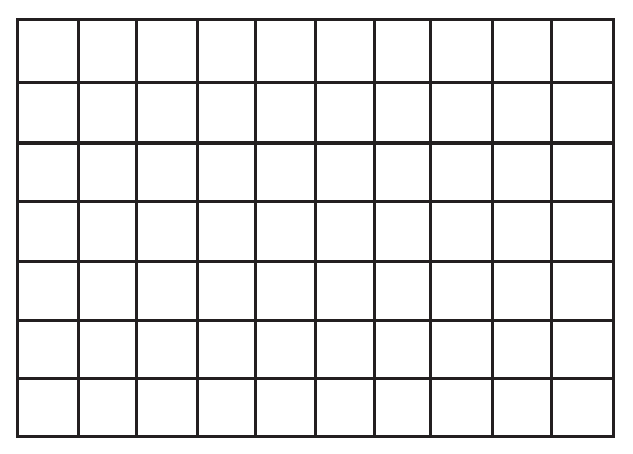
\includegraphics[width=0.3\textwidth]{images/m_regular_mesh}
	}
	\hspace{10mm}
	\subfigure[Malha não regular topologicamente estruturada]
	{
		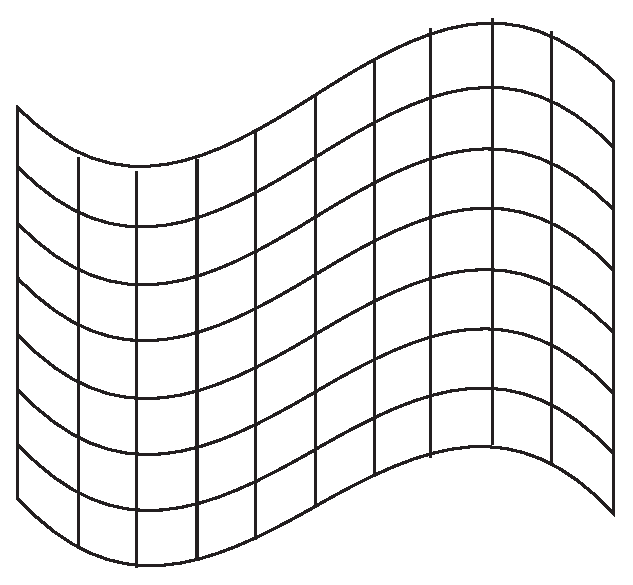
\includegraphics[width=0.3\textwidth]{images/m_irregular_mesh}
	}
	\caption{Tipos de malhas utilizadas nesta dissertação, em 2D.}
	\label{fig:meshes}
\end{figure}
    
\subsubsection{Malhas Regulares}
\label{subsec:my.struct}

\begin{figure}[h]
	\centering
	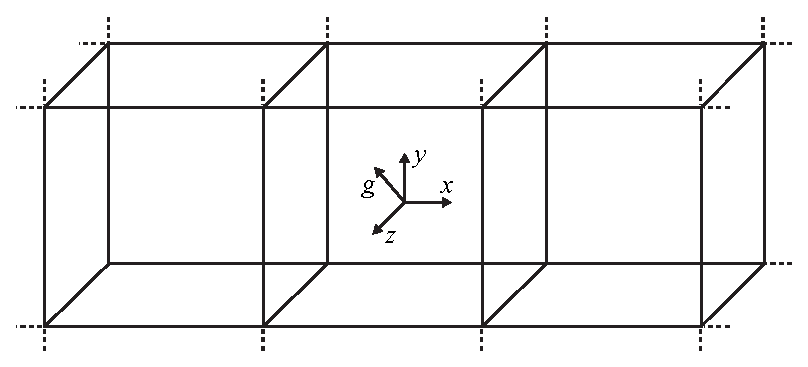
\includegraphics[width=0.7\textwidth]{images/m_regular_cells}
	\caption{Exemplo de células em malhas regulares.}
	\label{fig:m_regular_cells}
\end{figure}

	O método de diferenças finitas descreve como obter uma aproximação polinomial para a derivada de uma função $ f $ em um determinado ponto $ p $, utilizando $ n $ amostras de $ f $ equidistantes entre si a uma distância $ h $. Logo, o método das diferenças finitas pode ser utilizado para calcular as derivadas dos volumes com malhas regulares, uma vez que a distância entre suas células é sempre a mesma, na direção dos eixos.
	
	Nessa dissertação, optou-se por utilizar diferença central com $ n = 3 $. Isto é, uma das amostras é o próprio ponto $ p $ onde se deseja avaliar a derivada. As outras duas, estão a $ +h $ e $ -h $ de $ p $. A Equação~\eqref{eq:diff} mostra a primeira derivada de uma função $ f $ em um dado ponto $ p $, através de diferenças finitas centrais, como descrito acima.
	
\begin{equation}\label{eq:diff}
	f'(p) = \frac{f(p + h) - f(p - h)}{2h}
\end{equation} \

	Escolhendo o menor $ h $ discreto possível, a aplicação dessa equação no volume de dados implica em: para todas as posições do volume, computar a diferença entre os dois vizinhos mais próximos em uma mesma direção, dividido pela distância entre os mesmos. No entanto, como explicado na Seção~\ref{sec:gordon.bound}, as derivadas devem ser calculadas na direção do gradiente.
	
	O gradiente de uma função é um vetor formado pelas derivadas parciais dessa função, como indica a Equação~\eqref{eq:grad}. Assim, para cada posição do volume, o vetor gradiente também pode ser recuperado através da Equação~\eqref{eq:diff}, aproximando as derivadas nas direções $ x $, $ y $ e $ z $. Contudo, utilizar a Equação~\eqref{eq:diff} na direção do gradiente para cada posição do volume não é uma tarefa trivial, já que há apenas 3 direções do volume na qual as amostras podem ser igualmente espaçadas entre si. É preciso então recorrer à propriedade do cálculo vetorial de que a derivada direcional em uma dada direção é igual ao produto escalar do gradiente da função com o vetor da direção, como mostra a Equação~\eqref{eq:ddir}.
	
\begin{equation}\label{eq:grad}
	\nabla f = \bigg(\frac{\partial f}{\partial x}, \frac{\partial f}{\partial y}, \frac{\partial f}{\partial z}\bigg)
\end{equation} \

\begin{equation}\label{eq:ddir}
D_{\widehat{u}} f = \nabla f \cdot \widehat{u}
\end{equation} \

	Logo, a derivada na direção do gradiente é a própria norma do gradiente:

\begin{equation}\label{eq:first_derivative}
	D_{\widehat{\nabla f}} f = \nabla f \cdot \widehat{\nabla f} = \nabla f \cdot \frac{\nabla f}{\|\nabla f\|} = \|\nabla f\|
\end{equation} \

	Não é possível calcular a terceira derivada diretamente, utilizando os conceitos acima. Porém, se a magnitude do gradiente for armazenada em um novo campo escalar, a Equação~\eqref{eq:first_derivative} pode ser aplicada novamente, agora sobre $ \|\nabla f\| $. Com isso, obtém-se a segunda derivada do volume, a partir da qual pode se obter a terceira, repetindo o mesmo processo. As equações abaixo formalizam o cálculo da segunda e terceira derivadas, na direção do gradiente. 
	
	Com o fim de simplificar a compreensão das expressões, tomou-se a liberdade de representar o resultado da segunda derivada por $ \beta $.
	
\begin{align}
	\label{eq:second_derivative}
	D^{2}_{\widehat{\nabla f}} f & = D_{\widehat{\nabla f}} (\|\nabla f\|) = \nabla (\|\nabla f\|) \cdot \widehat{\nabla f} = \nabla (\|\nabla f\|) \cdot \frac{\nabla f}{\|\nabla f\|} = \beta \\
	\label{eq:third_derivative}
	D^{3}_{\widehat{\nabla f}} f & = D_{\widehat{\nabla f}} (\beta) = \nabla (\beta) \cdot \widehat{\nabla f} = \nabla (\beta) \cdot \frac{\nabla f}{\|\nabla f\|}
\end{align} \

	Antes de aplicar os conceitos discutidos até aqui, armazena-se em cada vértice a média da intensidade das células que o compartilham. Em seguida, é atribuído ao centro de cada face a média do valor dos vértices que a compõem. Dessa forma, o método de diferenças finitas é calculado entre os centros das faces de uma célula. Essa escolha faz com que o cálculo das derivadas seja igual, mesmo nas bordas do volume. Esse processo que interpola o valor escalar do centro de uma célula até o centro de suas faces é ilustrado na Figura~\ref{fig:m_cubes}.
	
\begin{figure}[h]
	\centering
	\subfigure[]
	{
		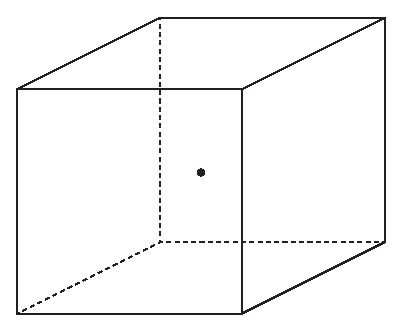
\includegraphics[width=0.25\textwidth]{images/m_cube}
	}
	\subfigure[]
	{
		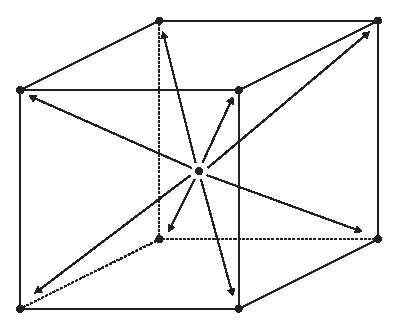
\includegraphics[width=0.25\textwidth]{images/m_cube_vertex}
	}
	\subfigure[]
	{
		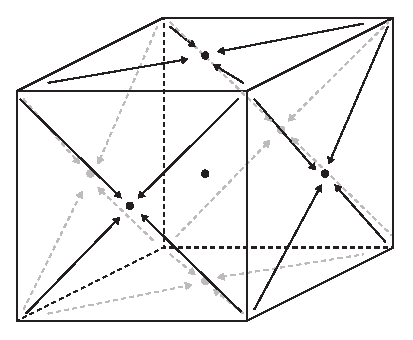
\includegraphics[width=0.25\textwidth]{images/m_cube_face}
	}
	\caption{Interpolação de valores do centro da célula para o centro das faces.}
	\label{fig:m_cubes}
\end{figure}
	
	Em posse dos valores escalares no centro das faces, a Equação~\eqref{eq:diff} é utilizada nas direções $ x $, $ y $ e $ z $, compondo respectivamente as componentes $ \frac{\partial f}{\partial x} $, $ \frac{\partial f}{\partial y} $ e $ \frac{\partial f}{\partial z} $ do gradiente $ \nabla f $. Então, a Equação~\eqref{eq:first_derivative} é aplicada e o resultado é armazenado no centro da célula, resultando no campo escalar da primeira derivada do volume. 
	
	Depois que a primeira derivada é calculada para todo o volume, a norma do gradiente armazenada no centro da célula é interpolada para o centro das faces através do mesmo processo descrito anteriormente. O vetor gradiente de cada célula já foi calculado na etapa anterior, então, pode-se aplicar a Equação~\eqref{eq:second_derivative} para obter a segunda derivada. Por fim, o resultado dessa iteração é interpolado para o centro das faces da mesma maneira, para que a terceira derivada seja calculada, de acordo com a Equação~\eqref{eq:third_derivative}.

\subsubsection{Malhas Não Regulares Topologicamente Estruturadas}
\label{subsec:my.nonstruct}

\begin{figure}[h]
	\centering
	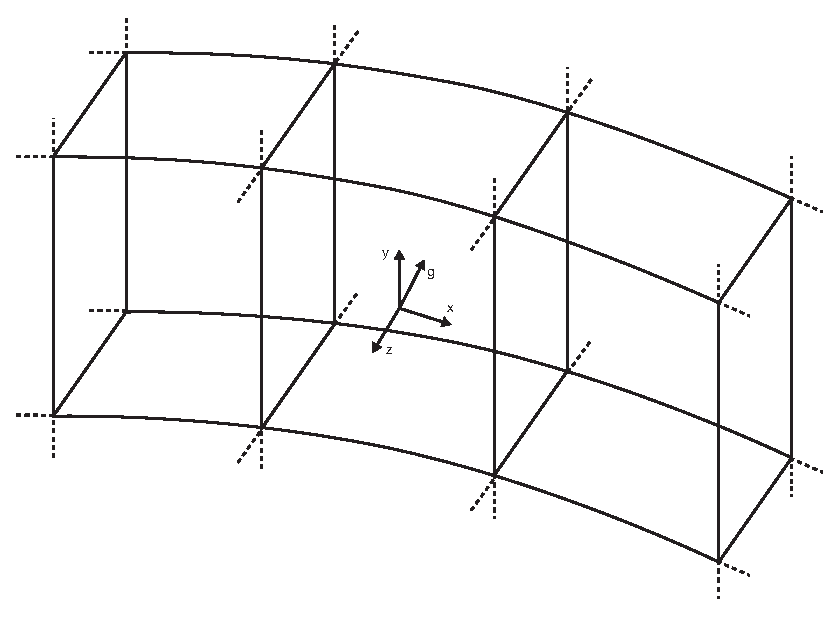
\includegraphics[width=0.6\textwidth]{images/m_irregular_cells}
	\caption{Exemplo de células em malhas não regulares topologicamente estruturadas.}
	\label{fig:m_irregular_cells}
\end{figure}

	Em malhas não regulares, a direção dos vivinhos mais próximos pode sempre variar de uma célula para outra. Portanto, a aplicação do método de diferenças finitas resultaria em derivadas direcionais distintas para cada célula, tornando inviável o uso dos conceitos apresentados até aqui. Contudo, é possível transformar o gradiente calculado no espaço paramétrico da malha, para o espaço cartesiano, como feito por \textit{Barroso et al.}~\cite{barata}.
	
	Aplicando a regra da cadeia, o vetor gradiente no espaço paramétrico $ \nabla f_{(s, t, p)} $ pode ser escrito em função do vetor gradiente no espaço cartesiano $ \nabla f_{(x, y, z)} $, como mostra a Equação~\eqref{eq:cadeia}. As derivadas parciais que relacionam os dois vetores, equivalem aos termos da matriz Jacobiana do espaço paramétrico. Então, a transformação entre os espaços pode ser expressa de forma reduzida pela Equação~\eqref{eq:cadeia_jacob}.
	\\
	
\begin{equation}\label{eq:cadeia}
	\nabla f_{(s, t, p)} = \left(
	\begin{array}{ccc}
		\vspace{1mm} \frac{\partial f}{\partial s} \\
		\vspace{1mm} \frac{\partial f}{\partial t} \\
		\frac{\partial f}{\partial p}
	\end{array}
	\right)
	 = \left(
	\begin{array}{ccc}
		\vspace{1mm}
		\frac{\partial f}{\partial x}\frac{\partial x}{\partial s} + \frac{\partial f}{\partial y}\frac{\partial y}{\partial s} + \frac{\partial f}{\partial z}\frac{\partial z}{\partial s}
		\\
		\vspace{1mm}
		\frac{\partial f}{\partial x}\frac{\partial x}{\partial t} + \frac{\partial f}{\partial y}\frac{\partial y}{\partial t} + \frac{\partial f}{\partial z}\frac{\partial z}{\partial t}
		\\
		\frac{\partial f}{\partial x}\frac{\partial x}{\partial p} + \frac{\partial f}{\partial y}\frac{\partial y}{\partial p} + \frac{\partial f}{\partial z}\frac{\partial z}{\partial p}
	\end{array}
	\right)
\end{equation} \

\begin{equation}\label{eq:jacob}
	J = 
	\begin{bmatrix}
	\frac{\partial x}{\partial s} && \frac{\partial y}{\partial s} && \frac{\partial z}{\partial s} \\
	\frac{\partial x}{\partial t} && \frac{\partial y}{\partial t} && \frac{\partial z}{\partial t} \\
	\frac{\partial x}{\partial p} && \frac{\partial y}{\partial p} && \frac{\partial z}{\partial p}
	\end{bmatrix}
\end{equation} \

\begin{equation}\label{eq:cadeia_jacob}
	\nabla f_{(s, t, p)} = J\ \nabla f_{(x, y, z)}
\end{equation} \

	De forma análoga, multiplicando a equação acima pela matriz Jacobiana inversa obtém-se:
	
\begin{equation}\label{eq:cadeia_jacob_inv}
	\nabla f_{(x, y, z)} = J^{-1}\ \nabla f_{(s, t, p)}
\end{equation} \

	A matriz Jacobiana e sua inversa devem ser calculadas para o centro $ C_{i, j, k} $ de cada célula. Abaixo, $ J $ é reescrita em função dos centros das faces, onde $ C_{i + \frac{1}{2}, j, k} $ indica o centro da face entre $ C_{i, j, k} $ e $ C_{i + 1, j, k} $.

\begin{equation}\label{eq:jacob_cell}
	J = 
\begin{bmatrix}
	C_{i + \frac{1}{2}, j, k} - C_{i - \frac{1}{2}, j, k}\\
	C_{i, j + \frac{1}{2}, k} - C_{i, j - \frac{1}{2}, k}\\
	C_{i, j, k + \frac{1}{2}} - C_{i, j, k - \frac{1}{2}}
\end{bmatrix}	
\end{equation} \

	Uma vez transformado para o espaço cartesiano, o vetor gradiente pode ser armazenado na célula. Então, o mesmo processo descrito na seção anterior ocorre: a magnitude do gradiente é interpolada até o centro das faces para que a próxima derivada possa ser calculada. Para obter a segunda e terceira derivadas, transforma-se para o espaço cartesiano o gradiente do campo escalar correspondente à derivada de menor ordem. Abaixo, as expressões para a primeira, segunda e terceira derivadas são reescritas com a correção para o espaço cartesiano:
	
\begin{equation}\label{eq:derivatives_cart}
\begin{aligned}
	\vspace{4mm}
	D_{\widehat{\nabla f}} f_{(x,y,z)} & = 
		J^{-1}\ \nabla f_{(s,t,p)} 
		\cdot 
		J^{-1}\ \widehat{\nabla f}_{(s,t,p)}
		= \|\nabla f_{(x,y,z)}\|
		\\
	\vspace{4mm}
	D^{2}_{\widehat{\nabla f}} f_{(x,y,z)} & = 
		J^{-1}\ \nabla (\|\nabla f_{(x,y,z)}\|)_{(s,t,p)}
		\cdot
		J^{-1}\ \widehat{\nabla f}_{(s,t,p)}
		= \beta
		\\
	D^{3}_{\widehat{\nabla f}} f_{(x,y,z)} & = 
	J^{-1}\ \nabla (\beta)_{(s,t,p)}
	\cdot
	J^{-1}\ \widehat{\nabla f}_{(s,t,p)}
\end{aligned}
\end{equation}

\section{Geração da função de transferência}
\label{sec:my.tf}
	Após calcular as derivadas para todas as células do volume, obtém-se a média da terceira derivada para cada $ v $ (já quantizado) do volume, dando origem a $ t(v) $. Essa função naturalmente possui um perfil serrilhado, uma vez que ela é formada pela média de valores quantizados. Então, convolui-se $ t(v) $ com uma gaussiana, para suavizá-la. Por fim, a função é normalizada, dividindo-a pelo seu maior valor absoluto.
	
	É importante enfatizar que esse processo, apesar de simples, é muito importante. Se a função $ t(v) $ tiver perfil serrilhado, ou não for suavizada suficientemente, seus pequenos extremos locais, isto é, aqueles que pouco diferem da sua vizinhança em amplitude, contribuem para uma função de transferência que realça mais isosuperfícies que a quantidade real de fronteiras existentes.

	Uma vez que o objetivo desta dissertação é automatizar a geração da FT, optou-se por definir um número fixo e suficiente de vezes que a função $ t(v) $ deve ser convoluída com a gaussiana. Essa decisão foi possível devido ao fato de que uma suavização em excesso altera pouco a função de transferência, se comparada com uma suavização ideal ou suficiente (todas feitas por uma função gaussiana). Então, foi decidido convoluir $ t(v) $ com uma função gaussiana $ 20 $ vezes, pois verificou-se que este valor é suficiente (ou mais), para todos os volumes avaliados no decorrer da pesquisa.
	
	Como discutido anteriormente, os mínimos locais em $ t(v) $ indicam fronteiras a serem realçadas. Portanto, todo centro de fronteira é determinado por um valor $ v_{f} $ tal que $t(v_{f}) < t(v_{f} - 1)$ e $ t(v_{f}) < t(v_{f} + 1)$. A contribuição de uma fronteira para a função de transferência é dada por uma gaussiana cuja amplitude máxima é $ |t(v_{f})| $. A espessura da gaussiana, aproximada por $ 2\sigma $, é um parâmetro que pode ser controlado pelo usuário e é inicializado com $ 2 $.
	
	Um fator de opacidade máximo $ \alpha_{max} $ foi definido para controlar melhor a transparência final da visualização. Dessa forma, o usuário possui um controle fino sobre a função de transferência, semelhante à função $ b(x) $ de \textit{Kindlmann e Durkin}~\cite{gordon}, porém, esse controle está implícito no modelo da função de transferência através de $ \sigma $ e $ \alpha_{max} $, como mostra a Equação~\eqref{eq:ft}.

\begin{equation} \label{eq:ft}
	\alpha(v) = \alpha_{max}\max_{\forall v_{f}}\big\{|t(v_{f})|e^{-\frac{(v-v_{f})^{2}}{2\sigma^{2}}}\big\}
\end{equation}\

	Como a função de transferência é composta por um conjunto de gaussianas centradas nos valores que correspondem às fronteiras, essas gaussianas podem ser subtraídas da FT, permitindo ao usuário visualizar apenas as fronteiras que desejar. Então, uma interface foi desenvolvida para permitir ao usuário visualizar o volume utilizando a FT gerada automaticamente, bem como aplicar a ela essas transformações.
	
	A Figura~\ref{fig:m_interface}~\ref{fig:m_interface_methods} mostra que a interface permite também alternar entre os seguintes métodos para geração automática de FTs:
	\begin{itemize}
		\item \quote{Our Method} $ \rightarrow $ Método proposto por esta dissertação.
		\item \quote{KD Method} $ \rightarrow $ Método 1D de \textit{Kindlmann e Durkin}~\cite{gordon}.
	\end{itemize}
	
	Caso o primeiro método seja selecionado, o usuário pode escolher quais fronteiras deseja visualizar. Para isso, sempre que um novo modelo é carregado, o componente exibido na Figura~\ref{fig:m_interface}~\ref{fig:m_interface_iso} é recarregado com uma lista de valores do volume nos quais há ocorrência de fronteira. Então, o usuário pode alternar entre visualizar todas (\quote{Select all}), nenhuma (\quote{Select None}), ou um conjunto específico a partir da lista apresentada.
	
	É possível ainda alternar para o modo de isovolume. Nele apenas um valor de intensidade pode ser escolhido na lista, pois a função de transferência será máxima em todos os valores superiores ao escolhido (\quote{+ IsoVolume +}), ou inferiores (\quote{- IsoVolume -}). Contudo, se o método selecionado for o \quote{KD Method}, as opções discutidas são desabilitadas.
	
	A Figura~\ref{fig:m_interface}~\ref{fig:m_interface_bx} mostra componentes da interface que estão sempre habilitados. Para o método de \textit{Kindlmann e Durkin}~\cite{gordon}, esses controles definem a própria função $ b(x) $, onde \quote{Thickness} define a largura da função gaussiana enquanto sua altura é definida pela multiplicação de \quote{Opacity Factor} e \quote{Alpha}. Caso a função de transferência utilizada seja a definida pelo método proposto nesta dissertação, o parâmetro $ \alpha_{max} $ é obtido através do produto de \quote{Opacity Factor} com \quote{Alpha} e $ \sigma $ recebe o valor de \quote{Thickness}.
	
\begin{figure}[H]
	\centering
	\begin{tabular}{cc}
		\begin{tabular}{c}
			\subfigure[]
			{
				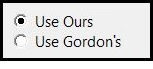
\includegraphics[width=0.21\textwidth]{images/m_interface_methods}
				\label{fig:m_interface_methods}
			}\\
			\subfigure[]
			{
				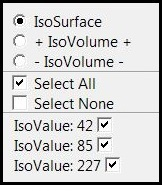
\includegraphics[width=0.21\textwidth]{images/m_interface_iso}
				\label{fig:m_interface_iso}
			}
		\end{tabular}
		&
		\begin{tabular}{c}
			\subfigure[]
			{
				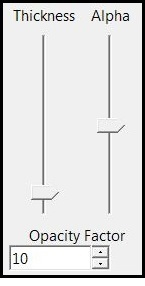
\includegraphics[width=0.2\textwidth]{images/m_interface_bx}
				\label{fig:m_interface_bx}
			}
		\end{tabular}
	\end{tabular}
	\caption{Campos da interface de controle do usuário.}
	\label{fig:m_interface}
\end{figure}

	Os controles da Figura~\ref{fig:m_interface} são referentes à função de transferência exibida na Figura~\ref{fig:m_interface_all}~\ref{fig:m_interface_all_tf}, cuja visualização do volume pode ser vista na Figura~\ref{fig:m_interface_all}~\ref{fig:m_interface_all_res}. Supondo uma interação do usuário com a interface, ainda sobre o mesmo volume, caso apenas a opção \quote{IsoValue 85} fosse marcada e o usuário aumentasse a largura da FT, o resultado seria a Figura~\ref{fig:m_interface_isoval}~\ref{fig:m_interface_iso_tf}. A visualização volumétrica correspondente ao uso dessa FT é exibida na Figura~\ref{fig:m_interface_isoval}~\ref{fig:m_interface_iso_res}.
	
\begin{figure}[h]
	\centering
	\subfigure[]
	{
		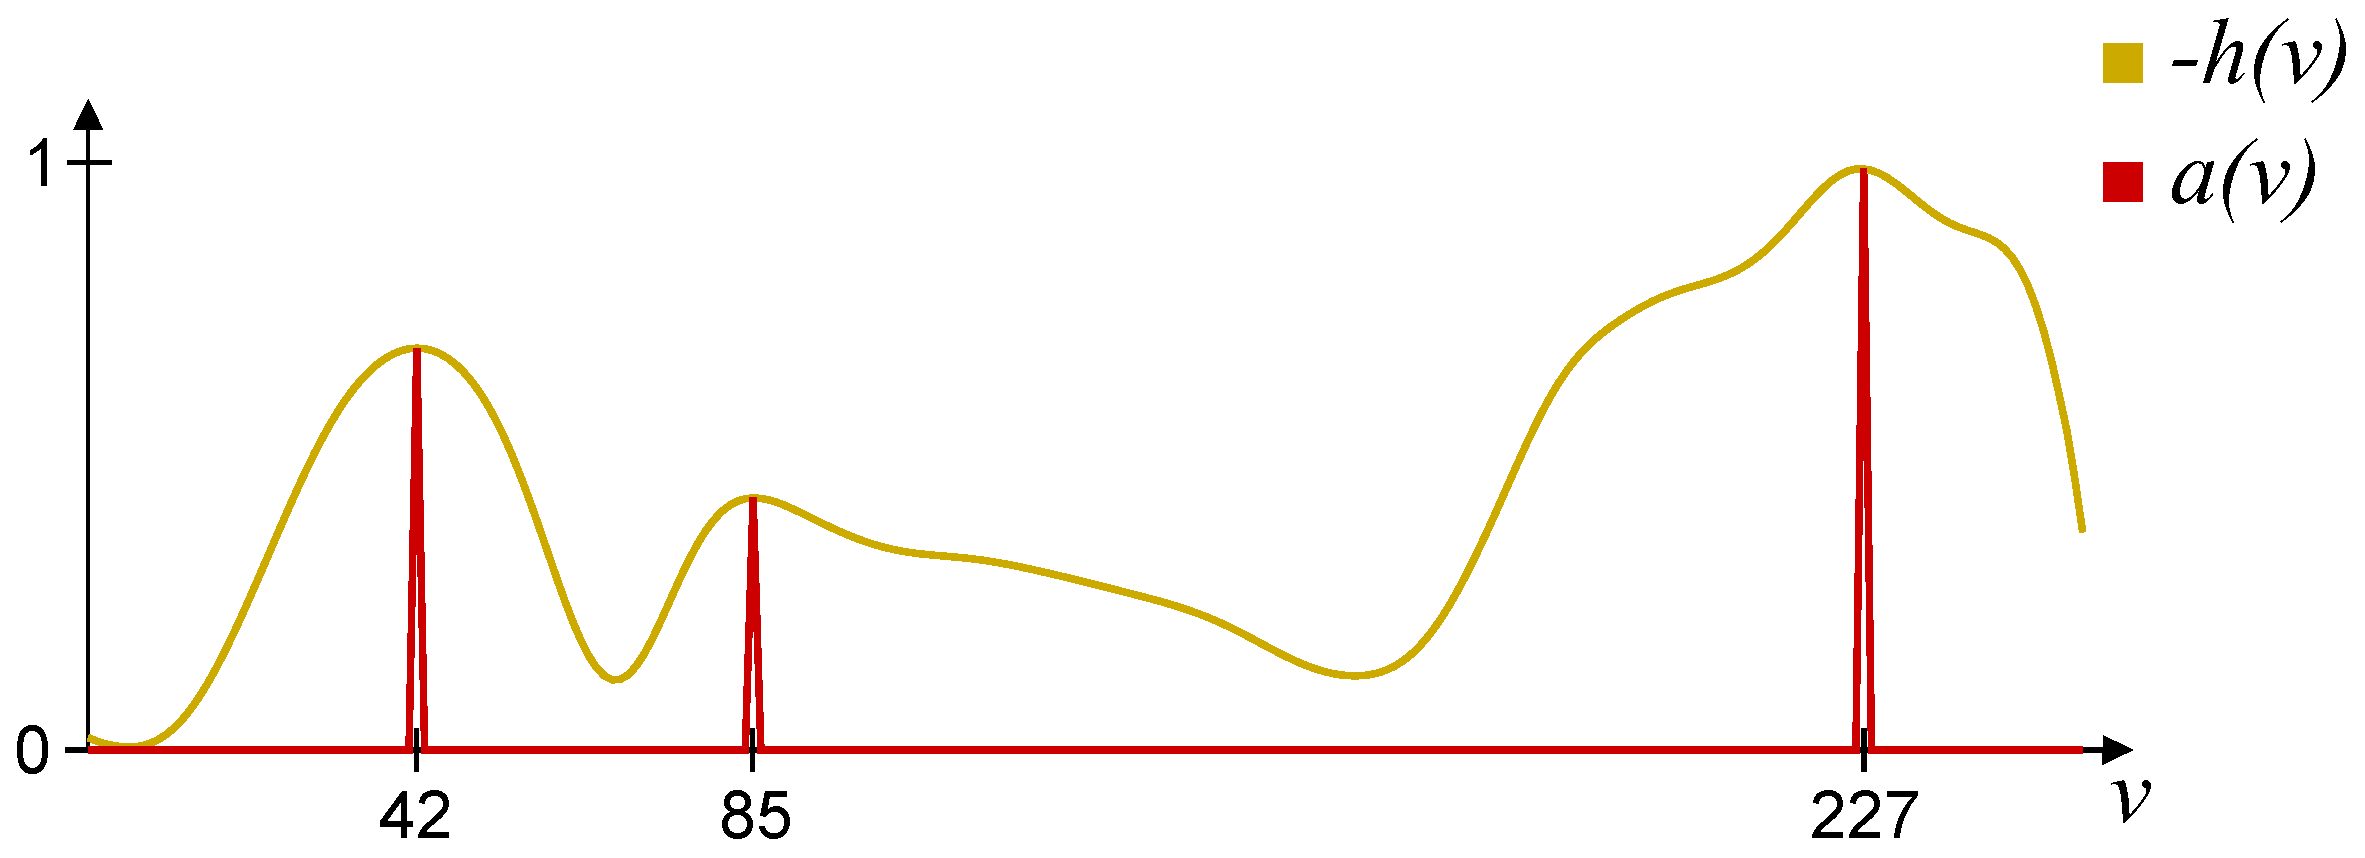
\includegraphics[width=1\textwidth]{images/m_interface_all}
		\label{fig:m_interface_all_tf}
	}
	\subfigure[]
	{
		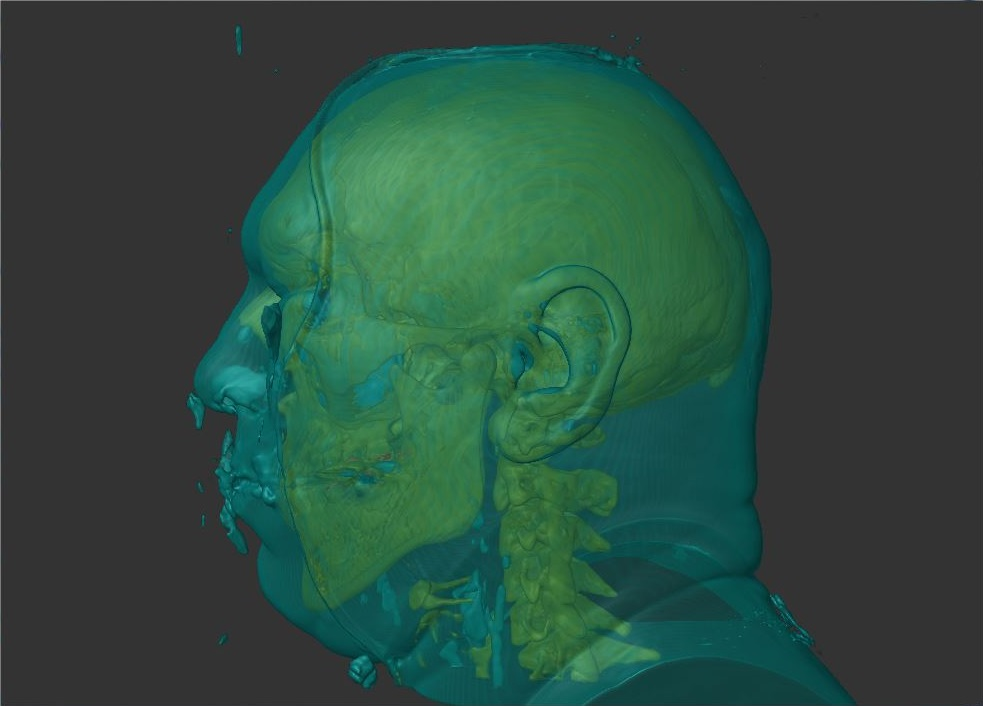
\includegraphics[width=0.8\textwidth]{images/m_interface_all_res}
		\label{fig:m_interface_all_res}
	}
	\caption{}
	\label{fig:m_interface_all}
\end{figure}

\begin{figure}[h]
	\centering
	\subfigure[]
	{
		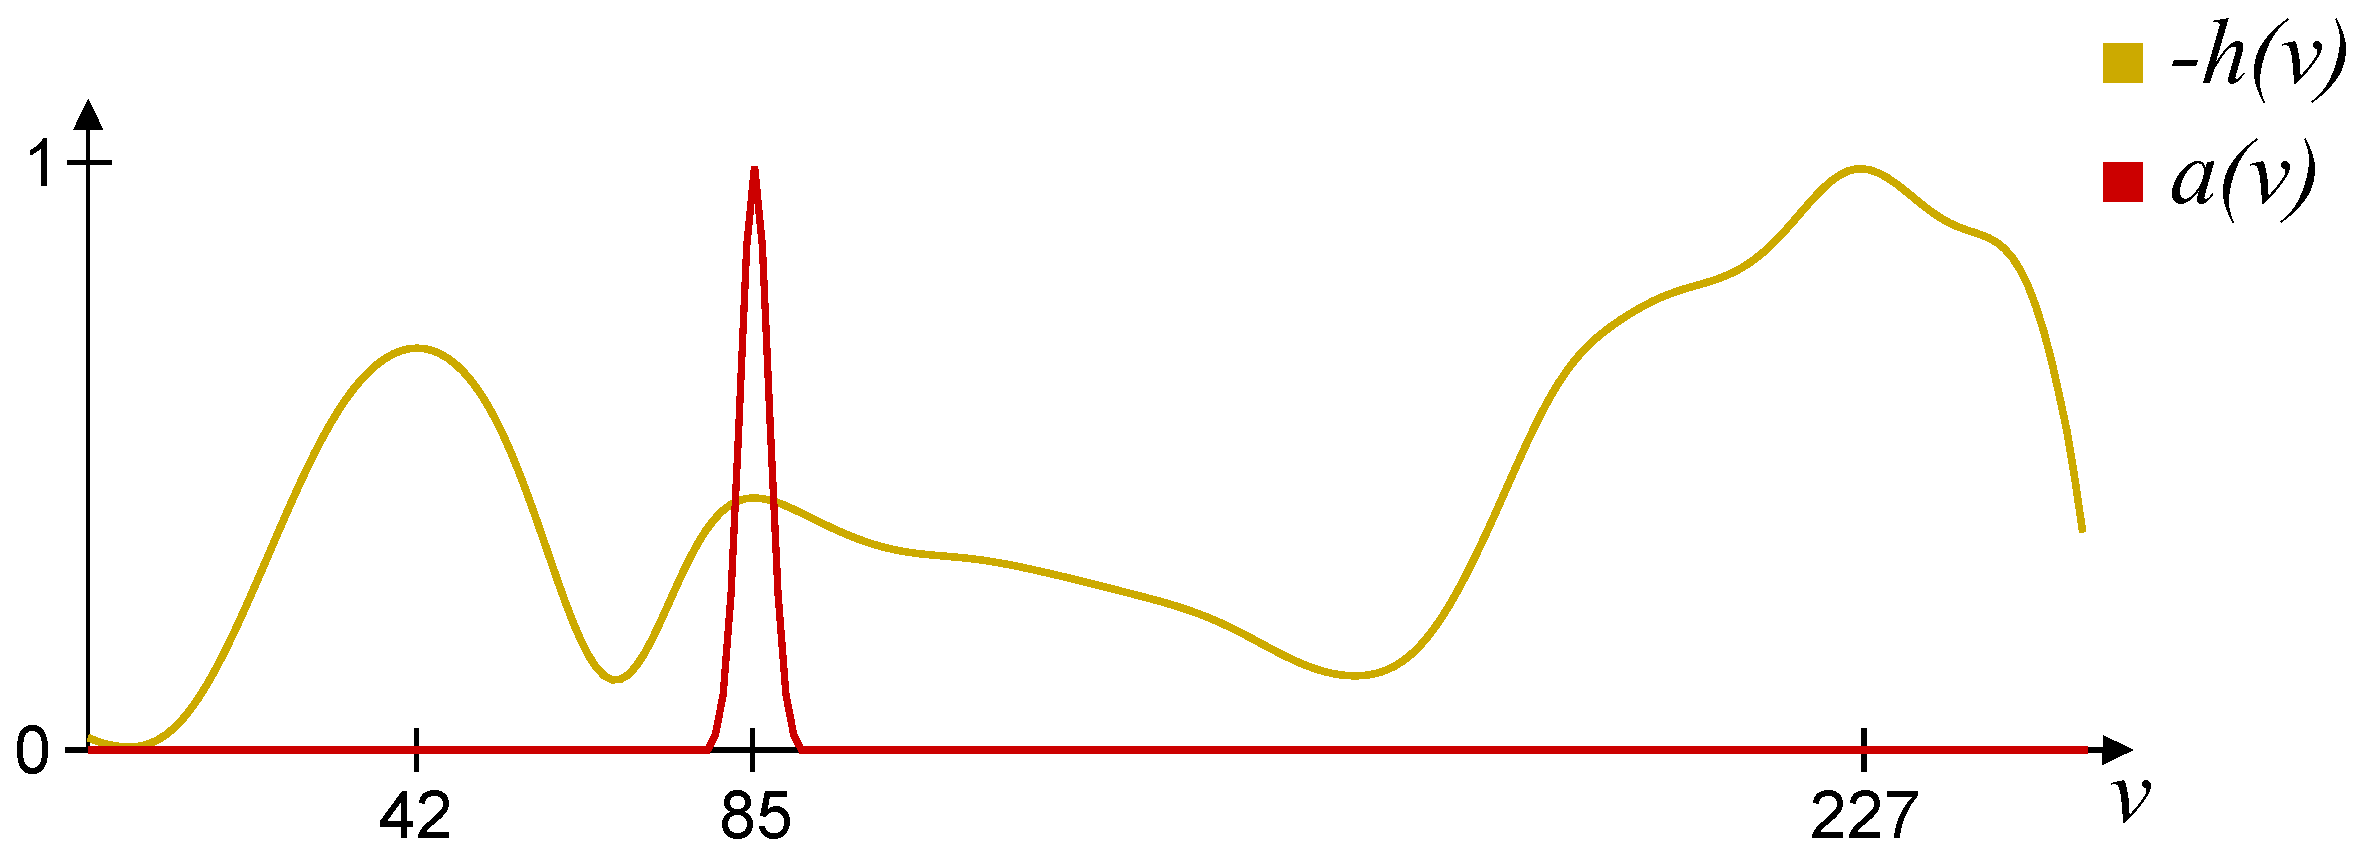
\includegraphics[width=1\textwidth]{images/m_interface_iso_tf}
		\label{fig:m_interface_iso_tf}
	}
	\subfigure[]
	{
		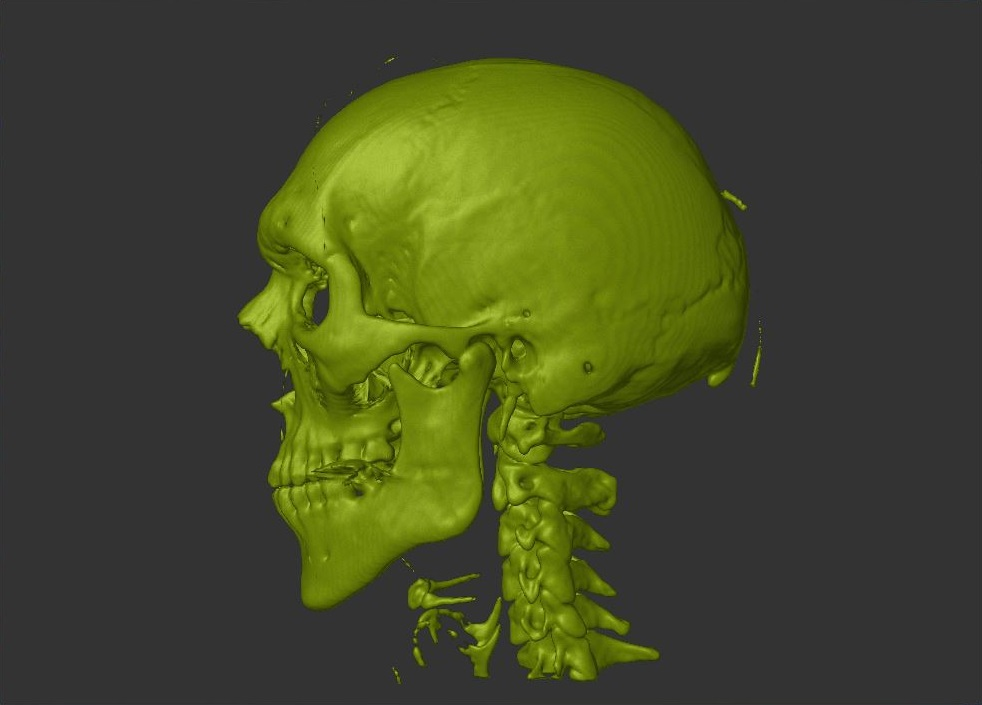
\includegraphics[width=0.7\textwidth]{images/m_interface_iso_res}
		\label{fig:m_interface_iso_res}
	}
	\caption{}
	\label{fig:m_interface_isoval}
\end{figure}